\hypertarget{target:chap4}{}\chapter{محاسبه حجم اجسام با استفاده از انتگرال}\label{chap:volume}

\section{حجم اجسام دورانی}
یکی از کاربردهای اصلی انتگرال معین، محاسبه حجم اجسام سه‌بعدی است که از دوران یک ناحیه حول یک محور ایجاد می‌شوند. اگر از روش دیسک استفاده کنیم، حجم حاصل از دوران تابع $f(x)$ حول محور $x$ در بازه $[a,b]$ بر اساس رابطه \eqref{eq:vol_formula} محاسبه خواهد شد:
\begin{equation}
	V = \pi \int_{a}^{b} [f(x)]^2 \, dx.
	\label{eq:vol_formula}
\end{equation}

برای درک بهتر نحوه عملکرد این مفهوم هندسی بر روی توابع خاص، تابع چندضابطه‌ای رابطه \eqref{eq:piecewise_int} را به عنوان نمونه در نظر بگیرید که رفتار هندسی منحنی مورد نظر را مشخص می‌کند:
\begin{equation}
	h(x) = 
	\begin{cases}
		\sqrt{x} & x \ge 0, \\
		0 & x < 0.
	\end{cases}
	\label{eq:piecewise_int}
\end{equation}

اگر این تابع تعریف شده در رابطه \eqref{eq:piecewise_int} را در بازه $[0,2]$ حول محور $x$ دوران دهیم، حجم جسم حاصل با استفاده از قضیه اساسی حسابان و جایگذاری ضابطه مربوطه، به صورت فرآیند محاسباتی شکسته و زنجیره‌ای در رابطه \eqref{eq:align_long} محاسبه می‌گردد:
\begin{align}
	V &= \pi \int_{0}^{2} (\sqrt{x})^2 \, dx \nonumber \\
	&= \pi \int_{0}^{2} x \, dx \nonumber \\
	&= \pi \left[ \frac{x^2}{2} \right]_{0}^{2} = \pi \left( \frac{4}{2} - 0 \right) = 2\pi.
	\label{eq:align_long}
\end{align}

همان‌طور که در روند حل رابطه \eqref{eq:align_long} مشخص است، انتگرال‌گیری روی ضابطه فعالِ تابع به یک جواب دقیق و مستقل ختم می‌شود.

\section{تحلیل گرافیکی و مقایسه کاربردها}
در شکل \ref{fig:comparison}، تصویر هندسی مربوط به مساحت زیر نمودار و فرآیند تولید دیسک‌های دورانی به عنوان دو زیرشکل مستقل چیده شده‌اند.

\begin{figure}[htbp]
	\centering
	\begin{subfigure}[b]{0.48\textwidth}
		\centering
		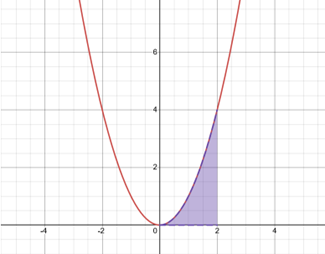
\includegraphics[width=\textwidth]{Images/Chapter3/Picture1.png} 
		\caption{مساحت زیر نمودار تابع $y=x^2$}
		\label{fig:sub_area}
	\end{subfigure}
	\hfill
	\begin{subfigure}[b]{0.48\textwidth}
		\centering
		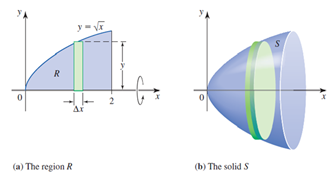
\includegraphics[width=\textwidth]{Images/Chapter4/Picture2.png} 
		\caption{ایجاد حجم دورانی با روش دیسک}
		\label{fig:sub_vol}
	\end{subfigure}
	\caption{نمودارهای توصیفی کاربرد انتگرال معین در محاسبات هندسی}
	\label{fig:comparison}
\end{figure}

با ارجاع به شکل \ref{fig:comparison}، می‌توان تفاوت ماهیت محاسبات مساحت در زیرشکل \ref{fig:sub_area} و حجم دورانی در زیرشکل \ref{fig:sub_vol} را دریافت. در نهایت، خلاصه‌ای از مقایسه این دو کاربرد در جدول \ref{td:compare} با رعایت استایل خط ضخیم و رنگ‌آمیزی آمده است.

\begin{table}[ht]
	\centering
	\caption{مقایسه کاربرد انتگرال در محاسبه مساحت و حجم}
	\label{td:compare}
	\renewcommand{\arraystretch}{1.5}
	\setlength{\tabcolsep}{10pt}
	\rowcolors{2}{blue!10}{white}
	\begin{tabular}{c!{\color{blue}\vrule width 1.5pt}c|c}
		\hline
		کاربرد & فرمول ریاضی & توضیح کاربردی \\
		\noalign{\hrule height 1.5pt}
		مساحت & $\int_{a}^{b} f(x) \, dx$ & محاسبه سطوح زیر یک یا بین دو منحنی پیوسته \\
		حجم & $\pi \int_{a}^{b} [f(x)]^2 \, dx$ & تعیین گنجایش اجسام حاصل از دوران حول محورها \\
		\hline
	\end{tabular}
\end{table}